\section{Chameleon Gravity}
\label{sec_cham}
We now describe \fR\ gravitites exhibiting the chameleon mechanism in more detail. As stated, this mechanism uses the large mass of the chameleon field in high density regions and chameleon gravity can satisfy tests of the equivalence principle in Solar System. The action of a chameleon scalar field $\chi$ in the Einstein frame is given by the action \eqref{eq:S_ein_fr}. Varying the action with respect to the field $\chi$ one can obtain the equation of motion
\eq{
	\label{eom:cham}
	\Box\chi=V_{,\chi}-\sum_i\frac{\beta_i}{\Mpl}e^{4\beta_i\chi/\Mpl}g^\uv_{(i)}T^{(i)}_\uv,
}
where $T^{(i)}_\uv$ is the stress-energy tensor for the $i$-th matter component. For a perfect isontropic fluid the equation of motion is
\eq{
	\Box\chi=V_{,\chi}+\sum_i(1-3w_i)\frac{\beta_i}{\Mpl}\rho_i e^{(1-3w_i)\beta_i\chi/\Mpl}.
}
This equation could be read as
\eq{
	\Box\chi=V_{\eff,\chi}\left(\chi\right),
}
where the effective potential $V_{\eff}$ is defined by
\eq{
	V_{\eff}\left(\chi\right)\equiv V(\chi)+\sum_i\rho_i e^{(1-3w_i)\beta_i\chi/\Mpl}.
}
If the couplings $\beta_i$ are the same for each matter component with the same $w$ (we can omit the radiation in the sum) and the overall density is $\rho=\sum_i\rho_i$, then the effective potential reads
\eq{
	V_{\eff}\left(\chi\right)\equiv V(\chi)+\rho e^{(1-3w)\beta\chi/\Mpl}.
}
For the quasi-static and weak $(\beta\chi/\Mpl\ll1)$ field in a weak gravity background (the Minkowski background) with non-relativistic matter, the equation further simplifies as
\eq{
	\label{eq:cham}
	\Delta \chi=\frac{\beta}{\Mpl}\rho+V_{,\chi},
}
which looks like the normal Poisson equation but with an extra non-linear term.
\subsection{Chameleon Force}
The interaction of the chameleon field with matter is described by the conformal coupling \eqref{eins_trans}. Free matter fields $\psi_m^{(i)}$ follow geodesics of the Jordan frame metric. In the Einstein frame they follow modified trajectories affected by the chameleon field \parencite{Waterhouse:2006wv}
\eq{
\frac{\dd^2x^\mu}{\dd\tau^2}+\Gamma^\mu_{\alpha\beta}\dddd{x^\alpha}{\tau}\dddd{x^\beta}{\tau}=-\frac{\beta_i}{\Mpl}\left(2\chi_{,\alpha}\dddd{x^\alpha}{\tau}\dddd{x^\mu}{\tau}+g^{\beta\mu}\chi_{,\beta}\right).
}
Note that the chameleon force violates the weak Equivalence Principle only if there exist two matter species with differing values of $\beta_i$. In the non-relativistic limit, a test particle of mass $m$ of species $i$ in a static chameleon field $\chi$ is moving under a force $\mb{F}_\chi$ given by
\eq{
\label{cham_force}
\frac{\mb{F}_\chi}{m}=-\frac{\beta_i}{\Mpl}\mb{\nabla}\chi
}
\subsection{Chameleon mechanism}
As discussed previously, we need some sort of a screening mechanism to avoid Solar System tests of GR. It means as seen from \eqref{cham_force} that the chameleon potential needs to approach some constant value in dense regions or at least have a marginally suppressed amplitude.

Suppose we have a background solution $\chi_0$ which minimizes the effective potential with $\rho=\rho_0$. For small fluctuations $\chi=\chi_0+\delta\chi$ and $\rho=\rho_0+\delta\rho$ we can linearized \eqref{eq:cham} to obain
\eq{
\label{eq:cham_lin}
\Delta \delta\chi=\frac{\beta}{\Mpl}\delta\rho+m^2_0\delta\chi,
}
where
\eq{
m^2_0\equiv V_{,\chi\chi}(\chi_0).
}
Except for the screening term the equation \eqref{eq:cham_lin} has the same behavior as the Poisson equation for the Newtonian potential $\Phi_N$. For a spherically symmetric density profile this gives solution
\eq{
\chi=\chi_0+2\beta\Mpl\Phi_N\left(r\right)e^{-m_0 r}.
}
As the objects in the background become more massive (larger and/or denser) the Newtonian potential grows larger (in magnitude) and so the deviation of $\chi$ from background solution $\chi_0$. At some point this deviation is no longer small and the potential term in \eqref{eq:cham} cannot be treated perturbatively. It starts canceling the first source term and eventually the field $\chi$ posses a new value which minimizes the effective potential inside an object.

This is the essence of the chameleon mechanism. Let us derive the mechanism in a more proper and exact way.
\subsection{Chameleon Profile}
\label{cham_prof}
To obtain the chameleon behavior described above we need to choose a chameleon potential $V(\chi)$ with the right properties. To have a screening mechanism in \eqref{eq:cham} we need $V_{,\chi}<0$ to cancel the source term and $V_{,\chi\chi}>0$ to have a real mass of the field and stable behavior of perturbations.

We wish to find a solution for spherically symmetric matter distributions of a single species of pressureless matter such that
\begin{equation*}
\rho(r)=
\begin{cases}
\rho_c & r<R_c \\
\rho_0 & r>R_c,
\end{cases}
\end{equation*}
where $\rho_c>\rho_0$. Further we define $\chi_c$ and $\chi_0$ with their masses $m_c$ and $m_0$ (the masses of small fluctuations about $\chi_c$ and $\chi_0$) such as
\begin{align*}
V_{\eff,\chi}\left(\chi_c\right)_{|\rho=\rho_c}&\equiv0	&	m^2_c&\equiv V_{\eff,\chi\chi}\left(\chi_c\right) \\
V_{\eff,\chi}\left(\chi_0\right)_{|\rho=\rho_0}&\equiv0	&	m^2_0&\equiv V_{\eff,\chi\chi}\left(\chi_0\right).
\end{align*}
In the background with low density, the curvature of the potential is much shallower, corresponding to a light scalar that mediates a long range force. Inside the object of high density, the scalar acquires a large mass, and the force shuts off.

In spherical coordinates assuming spherical symmetry, equation \eqref{eq:cham} becomes
\eq{
\label{eq_cham_r}
\frac{\dd^2\chi}{\dd r^2}+\frac{2}{r}\dddd{\chi}{r}=\frac{1}{r}\frac{\dd^2\left(r\chi\right)}{\dd r^2}=V_{,\chi}\left(\chi(r)\right)+\frac{\beta}{\Mpl}\rho(r).
}
We must impose two boundary conditions which are
\begin{align*}
\dddd{\chi}{r}(r=0)&=0 \\
\chi(r\rightarrow\infty)&=\chi_0.
\end{align*}
The first one corresponds to a non-singularity of the solution at the origin while the later one ensures that the chameleon force vanishes at the infinity (as $\dd\chi/\dd r\rightarrow0$).

The equation \eqref{eq_cham_r} drives the field $\chi$ toward the $\chi_0$ outside the object and toward $\chi_c$ inside the object. In order to solve \eqref{eq_cham_r} we must do several approximations. Outside the object we assume that the field sits near the extreme $\chi_0$ and we can linearized our equation
\eq{
\frac{1}{r}\frac{\dd^2\left(r\chi\right)}{\dd r^2}=m^2_0(\chi-\chi_0),
}
with the decaying solution
\eq{
\chi(r)=-\frac{\beta}{4\pi\Mpl}\frac{\tilde{M}}{r}e^{-m_0 r}+\chi_0.
}
Note that the integration constant $\tilde{M}$ is not generally the mass of the object $M_c$ as in the case of the Newtonian potential because it is determined by the field inside the object which has different behavior than the Newtonian potential. As we will see later, for small Newtonian potentials (in magnitude) this effective mass $\tilde{M}\approx M_c$ but as the potential grows larger part of the object`s mass is screened away $\tilde{M}< M_c$.

Inside the object we use one of the two approximations based on the initial value of $\chi_i\equiv\chi(0)$ -- either $\chi_i\approx\chi_c$ or $\chi_i\gg\chi_c$ .
\subsubsection{Thin-shell regime}
In the \textit{thin-shell} regime the field initially sits very close the minimum $\chi_c$, i.e. we require
\eq{
(\chi_i-\chi_c)/\chi_c\ll1.
}
The field is frozen near this value until the friction term is sufficiently small to allow the field to roll. This ``moment'' is denoted by $R_{roll}$. As soon as $\chi$ is displaced significantly from $\chi_c$ we may neglect the potential term in \eqref{eq_cham_r}. This gives us the solution
\eq{
\chi(r)=
\begin{cases}
\chi_c & 0<r<R_{roll} \\
\frac{\beta}{6\Mpl}\rho_cr^2+\frac{A}{r}+D & R_{roll}<r<R_c.
\end{cases}
}
We have boundary conditions coming from the requirement on matching $\chi$ and  $\dd\chi/\dd r$ at $R_{roll}$, namely: $\chi=\chi_c$ and $\dd\chi/\dd r=0$ at $r=r_{roll}$. This fixes our constants and the solution is
\eq{
\label{eq_thin}
\chi(r)=
\begin{cases}
\chi_c & 0<r<R_{roll} \\
\frac{\beta\rho_c}{3\Mpl}\left(\frac{r^2}{2}+\frac{R^3_{roll}}{r}\right)-\frac{\beta\rho_cR^2_{roll}}{2\Mpl}+\chi_c & R_{roll}<r<R_c.
\end{cases}
}
The approximation of separating the solution into the two regions only makes sense if $(R_c-R_{roll})/R_c\ll1$. Otherwise there is no clear separation between the two regions, and one needs a solution valid over the entire range $0<r<R_c$. In \autoref{sec:num_cham} we solve equation \eqref{eq_cham_r} numerically and we will check these approximations against numerical solutions.

With approximation $(R_c-R_{roll})/R_c\ll1$ we can determines the effective mass of the object $\tilde{M}$ from the requirement $\chi(R_c^-)=\chi(R_c^+)$ and $\dd\chi/\dd r(R_c^-)=\dd\chi/\dd r(R_c^+)$.
\eq{
\tilde{M}=\frac{3\Delta R_c}{R_c}M_c,
}
where
\eq{
\frac{\Delta R_c}{R_c}\equiv\frac{\chi_0-\chi_c}{6\beta\Mpl|\Phi_N(R_c)|}\approx\frac{R_c-R_{roll}}{R_c}\ll1.
}
This qualitative derivation of the thin-shell regime is using too much strong assumptions and can be done more precisely without ignoring some of the terms but then it is harder to see the principle of the thin-shell effect. For more details see e.g. \textcite{Tamaki:2008mf,2007PhRvD..75f3501M,Waterhouse:2006wv}.
\subsubsection{Thick-shell regime}
In the \textit{thick-shell} regime the field is initially sufficiently displaced from the minimum -- $\chi_i\gg\chi_c$ that it begins to roll almost immediately (no friction term). Hence the interior solution is most easily obtained by taking the $R_{roll}=0$ in \eqref{eq_thin} and replacing $\chi_c$ by $\chi_i$
\eq{
\label{eq_thick}
\chi(r)=\frac{\beta\rho_cr^2}{6\Mpl}+\chi_i\ \ \ 0<r<R_c.
}
By matching the interior and exterior solutions, we obtain
\eq{
\begin{split}
\chi_i &=\chi_0-3\beta\Mpl\Phi_N(R_c)\\
\tilde{M} &=M_c,
\end{split}
}
which is the linear regime with no screening. From the definition of $\Delta R_c/R_c$ we also obtain
\eq{
\frac{\Delta R_c}{R_c}\equiv\frac{\chi_0-\chi_c}{6\beta\Mpl|\Phi_N(R_c)|}>1.
}
\subsubsection{Thin-shell suppression factor}
The chameleon force outside the object (where experiments take place) comparing to the Newtonian force is
\eq{
\begin{split}
\label{eq_cham_suppression}
\frac{F_{thick}}{F_N}&=2\beta^2 \\
\frac{F_{thin}}{F_N}&=2\beta^2\frac{3\Mpl\left(\chi_0-\chi_c\right)}{\beta\rho_cR^2_c},
\end{split}
}
where we ignore the term $m_0 r\ll1$. Therefore for the coupling $\beta$ of order unity the chameleon force is as strong as gravity unless it is screened away by the thin-shell effect.
%%%%%%%%%%%%%%%%%%%%%%%%%%%%%%
% HU-SAWICKI
%%%%%%%%%%%%%%%%%%%%%%%%%%%%%%
\subsection{Hu-Sawicki \texorpdfstring{\textit{\lowercase{f}(R)}}{fR} Model}
We wish to study a class of $f(R)$ models that accelerate cosmic expansion at late times, without the cosmological constant, while satisfying both cosmological and Solar System tests. We consider the family of Hu-Sawicki $f(R)$ models \parencite{Hu-Saw}. The action of these models is given by \eqref{eq:S_fr} and $f(R)$ has a broken power-law form
\eq{
	f(R)=-M^2\frac{c_1(R/M^2)^m}{c_2(R/M^2)^m+1}\,,
}
where the mass scale $M^2\equiv\bar\rho_0/3\Mpl^2$, $m>0$, and $c_1$ and $c_2$ are dimensionless parameters such that at high redshifts \LCDM\ cosmology is restored.

The formulation of modified gravity in this frame leads to second-order differential equations of motion \eqref{eq:fR} for $R$ and fourth-order field equations for $g_\uv$. With a conformal transformation \eqref{eins_trans} we may rewrite these equation in the Einstein frame with second-order differentials only \parencite[see, e.g.,][]{CHIBA20031}. In the Einstein frame, the Hu-Sawicki models correspond to chameleon gravity with the potential
\eq{
	V(\chi) &= \Mpl^2\Lambda-\frac{\beta\bar\rho_0}{n\Mpl}\left(2\beta\Mpl\Phiscrz\right)^{1-n}\chi^n\,, \\
    V_{,\chi}(\chi) &= -\frac{\beta}{\Mpl}\bar\rho_0\left(\frac{2\beta\Mpl\Phiscrz}{\chi}\right)^{1-n}\,,
}
where $\beta=\sqrt{1/6}$ and the power-law exponent $n$ and screening potential $\Phiscrz$ are now the free parameters of the theory. The screening potential has the following relation to the present scalaron value in $f(R)$-gravity:
\eq{
    \Phiscrz=\frac{3}{2}\ln{(1+f_{R0})}\approx\frac{3}{2}f_{R0}.
}
The chameleon obeys the equation of motion \eqref{eom:cham} which reduces for our study case (non-relativstic pressureless matter) to
\eq{
\label{eq:cham_husa}
	\Delta \chi = \frac{\beta}{\Mpl}\rho - \frac{\beta}{\Mpl}\bar\rho_0\left(\frac{2\beta\Mpl\Phiscrz}{\chi}\right)^{1-n}
}

\subsection{Numerical solutions}
\label{sec:num_cham}
% \todo{Heyrovsky D.:

% \textit{The model choice is unusual, since the primary relevance of the chameleon field is away from highdensity regions, where it can mimic the effect of the cosmological constant. Nevertheless, it is a good idea to check if the chameleon field doesn’t interfere at these scales. In this context one should point out that for a galactic halo with a 10 kpc scale it does not make much sense to plot the rotation curve out to 300 kpc. Regarding the cosmological simulations, attempts to jointly solve a gravitational Nbody code with the Poisson-like chameleon equation do not look very promising. It might be better to use a gravitational hydrodynamic code, which solves similar types of PDEs.}
% }

In this section we will show results of results of numerical solutions of chameleon profile. Our algorithm for finding solutions to \eqref{eq_cham_r} uses the shooting method \parencite{10.5555/42249} and is based on the original algorithm of \textcite{mastersthesis_vrastil}. We further improve the code readibility and possible parametrization. The code is publically available at \todo{GitHub}.

\subsubsection{Spherical objects in background}
In \autoref{fig:starlike} \todo{describe potential}
\begin{figure}
	\centering
	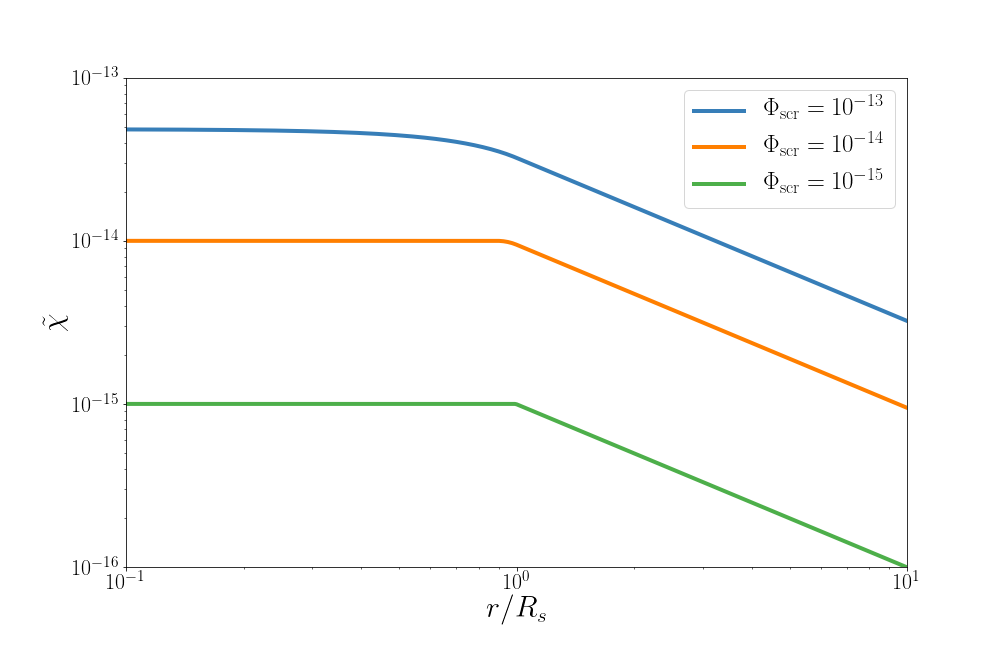
\includegraphics[width=1.0\linewidth]{{spherical_cham/starlike}.png}
	\caption{Chameleon profile for several screening potentials. The top solution is in the linear regime and is identical to the gravitainal potential. The other two solutions are in the screened regime and the amplitude of the field is suppressed.}
	\label{fig:starlike}
\end{figure}



In \autoref{fig:starlike_forces} \todo{describe forces}
\begin{figure}
	\centering
	
\includegraphics[width=1.0\linewidth]{{spherical_cham/starlike_forces}.png}
	\caption{Chameleon force relative to the standard gravitainal force for several screening potentials (given through the equivalence radius). For $R_{eq}\ll R_S$ there is no sreening outside the object. As the $R_{eq}$ grows the chameleon enters the screened regime.}
	\label{fig:starlike_forces}
\end{figure}

\subsubsection{NFW Halo}
In \autoref{fig:nfwlike_forces} \todo{describe forces}
\begin{figure}
	\centering
	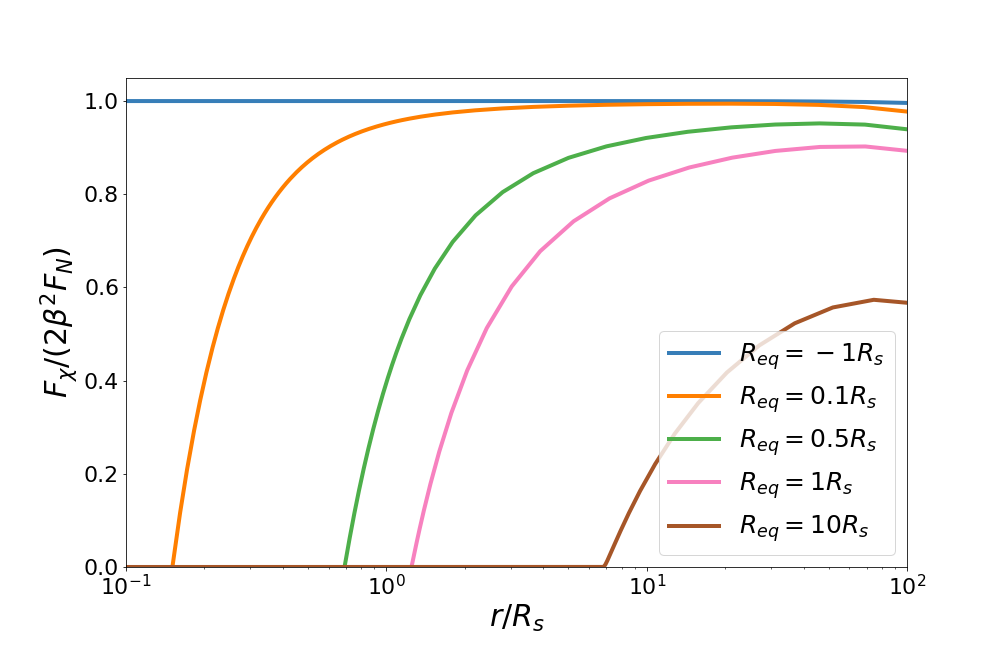
\includegraphics[width=1.0\linewidth]{{spherical_cham/nfwlike_forces}.png}
	\caption{Chameleon force relative to the standard gravitainal force for several screening potentials (given through the equivalence radius). For $R_{eq}\ll R_S$ there is no sreening outside the object. As the $R_{eq}$ grows the chameleon enters the screened regime.}
	\label{fig:nfwlike_forces}
\end{figure}


In \autoref{fig:nfwlike_pot_eff} \todo{describe effective screening potential}

\begin{figure*}
	\centering
		\begin{subfigure}{1.0\linewidth}
			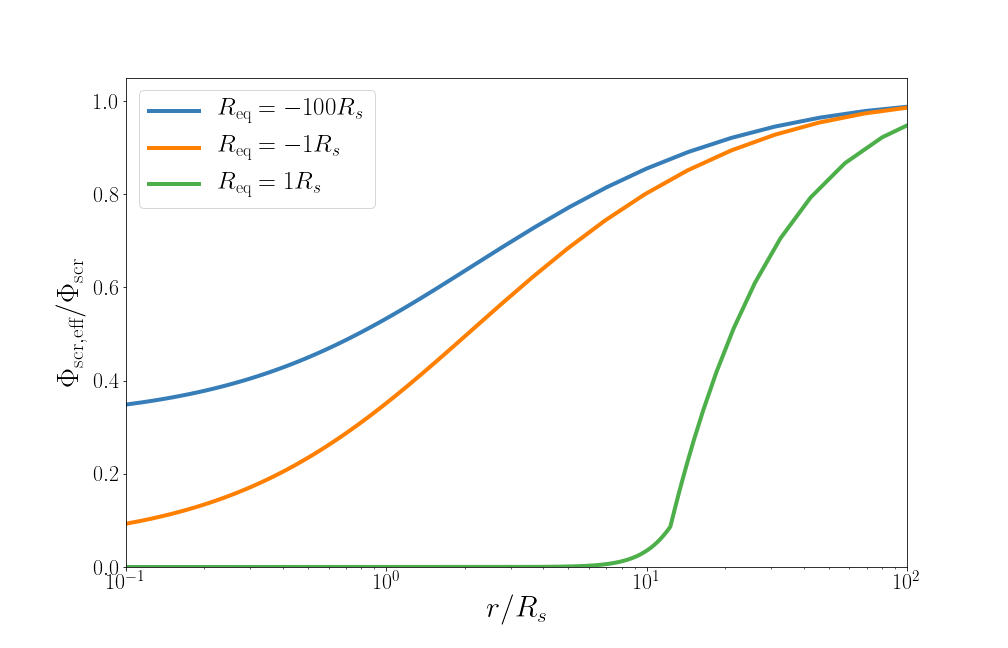
\includegraphics[width=1.0\linewidth]{{spherical_cham/nfwlike_pot_eff}.png}
		\end{subfigure}
		\begin{subfigure}{1.0\linewidth}
			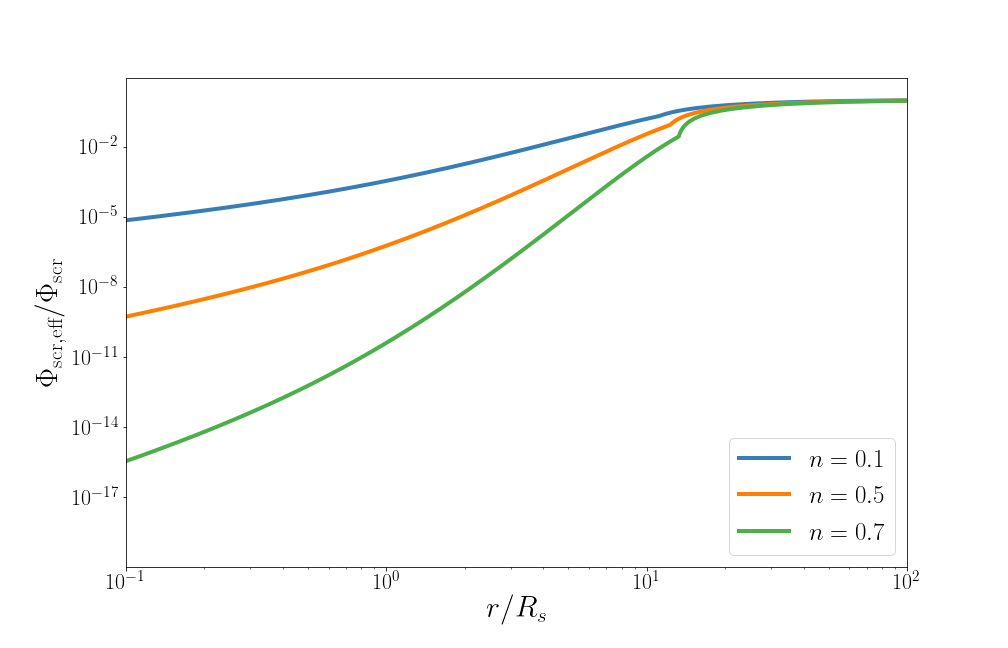
\includegraphics[width=1.0\linewidth]{{spherical_cham/nfwlike_pot_eff_n}.png}
		\end{subfigure}
		\caption{Effective screening potential relative to the screening potential for a cluster of galaxy, $M=10^{14} M_\odot, c=4$. Top Figure is shown for several screening potentials (given through the equivalence radius) while the bottom for different chameleon parameter $n$.}
		\label{fig:nfwlike_pot_eff}
\end{figure*}

In \autoref{fig:clustersYs} \todo{describe dynamical and lensing measurements}
\begin{figure*}
\begin{adjustwidth}{-3cm}{-1cm}
	\centering
		\begin{subfigure}{0.5\linewidth}
			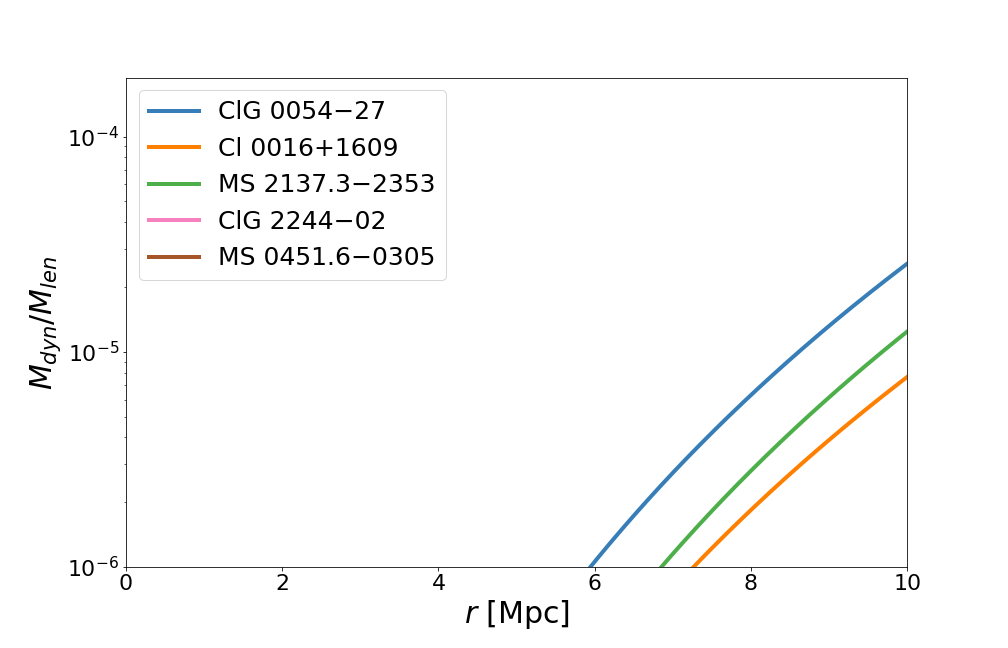
\includegraphics[width=1.0\linewidth]{{spherical_cham/clustersYs_-6}.png}
			\caption{$\Phiscr=10^{-6}$}
		\end{subfigure}%
		\begin{subfigure}{0.5\linewidth}
			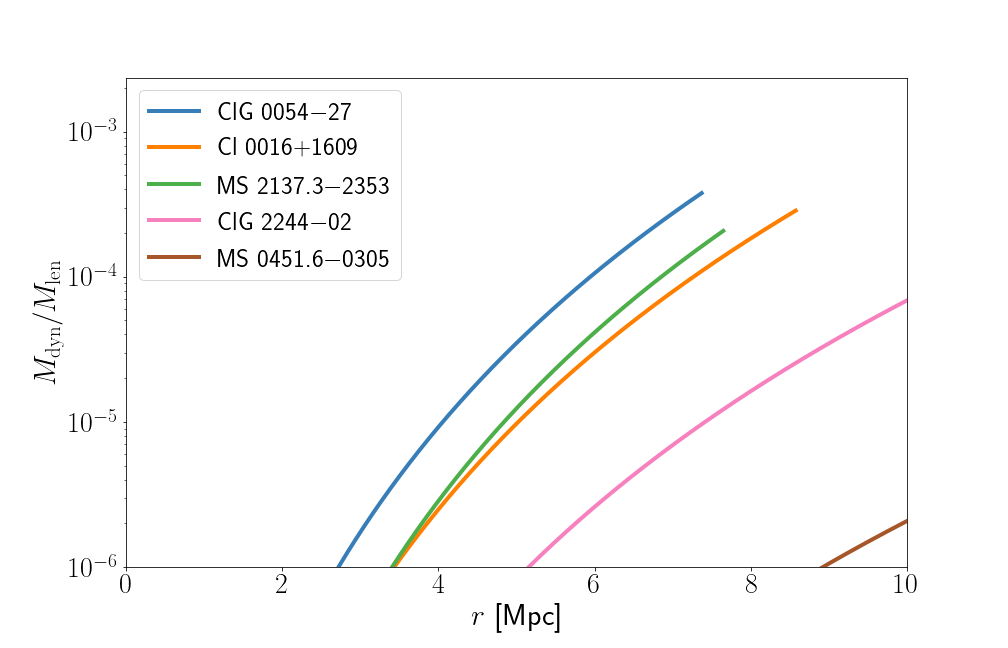
\includegraphics[width=1.0\linewidth]{{spherical_cham/clustersYs_-4}.png}
			\caption{$\Phiscr=10^{-4}$}
		\end{subfigure}
		\begin{subfigure}{0.5\linewidth}
			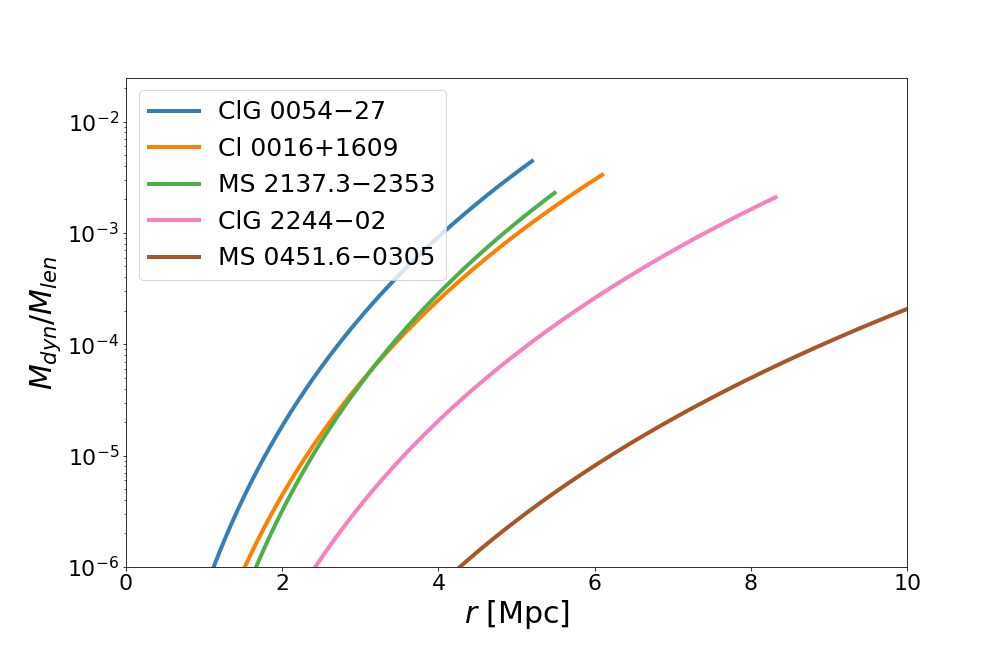
\includegraphics[width=1.0\linewidth]{{spherical_cham/clustersYs_-2}.png}
			\caption{$\Phiscr=10^{-2}$}
		\end{subfigure}%
		\begin{subfigure}{0.5\linewidth}
			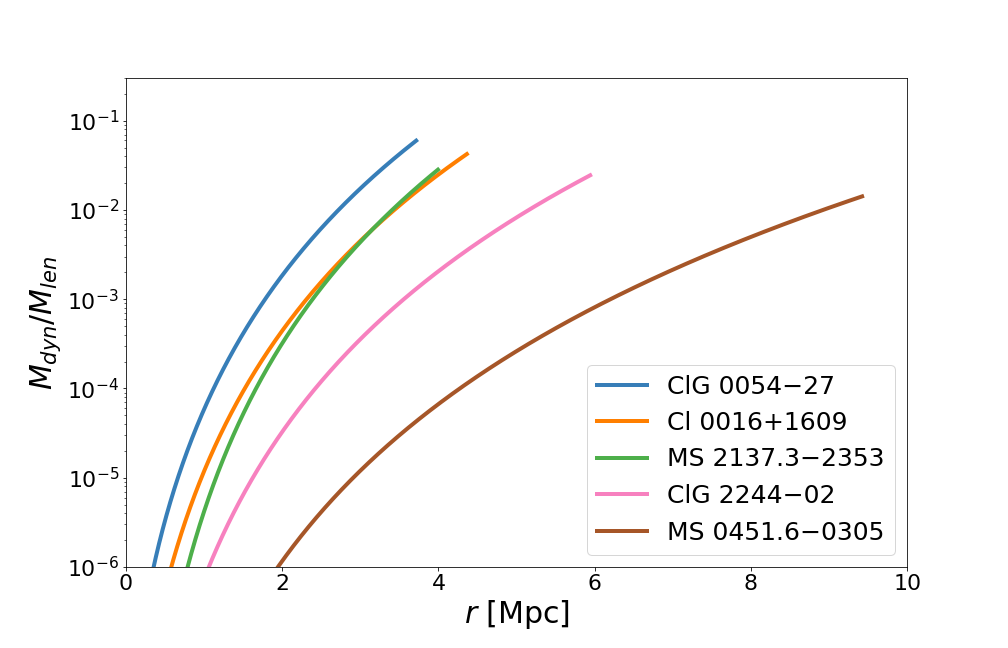
\includegraphics[width=1.0\linewidth]{{spherical_cham/clustersYs_0}.png}
			\caption{$\Phiscr=10^{0}$}
		\end{subfigure}
		\caption{Effective dynamical mass of the clusters relative to the actual (lensing) mass of the cluster. Cluster properties are: ClG 0054-27 $(c=1.2, M=0.42\cdot10^{14}M_\odot)$, Cl 0016+1609 $(c=2.1, M=1.12\cdot10^{14}M_\odot)$, MS 2137.3-2353 $(c=13, M=2.9\cdot10^{14}M_\odot)$, ClG 2244-02 $(c=4.3, M=4.5\cdot10^{14}M_\odot)$, MS 0451.6-0305 $(c=5.5, M=18\cdot10^{14}M_\odot)$. Parameters are taken from \textcite{2007MNRAS.379..190C}.}
		\label{fig:clustersYs}
\end{adjustwidth}
\end{figure*}